\section{Desarrollo y modelado}

En esta sección presentaremos las decisiones de diseño que tomamos para desarrollar la aplicación. Para esto, explicaremos las entidades del problema y se adjuntan diagramas de objetos, de clases y de secuencia para clarificar.

\subsection{Una simulación}

Como bien sabemos, una simulación se ejecutará en el momento en que un Participante envíe un reto y otro se lo acepte.

En ese sentido, en el contexto de un duelo, el participante elegirá el equipo que lo represente. Un equipo conocerá cinco jugadores (base,ala,escolta,ala pivote y pivote), un director técnico y un nombre. 

Cada jugador conocerá un conjunto de estadísticas que afectarán su rendimiento en el partido.
Cada técnico conocerá un libro de estrategias en donde estarán las posibles jugadas que hará su equipo durante la simulación.


\begin{center}
\includegraphics[height=140px, width=300px]{img/DC-Equipo.png} 
\end{center}


De esta forma, en el contexto de una simulación, tenemos 

\begin{center}
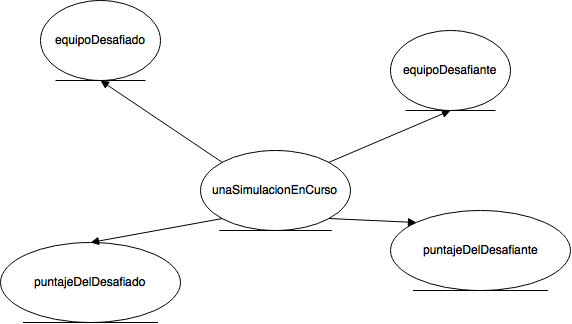
\includegraphics[height=140px, width=300px]{img/DO-SimulacionEnCurso.png} 
\end{center}


Una simulación tiene dos estados, en curso o terminada. Una en curso conoce el puntaje del desafiante y el desafiado, que luego cuando pase al estado de terminada, será el puntaje definitivo de la simulación.
Para modelar esto usamos el patrón State como muestra el siguiente diagrama de clases.

\begin{center}
\includegraphics[height=140px, width=300px]{img/DC-Simulacion.png}
\end{center}


Las posibles jugadas que pueden hacer los jugadores las modelamos con la idea de una Acción.
